 
$$ 20L = 2.9x+ 2.5y $$ 
Xotlil lives in Honduras and buys beans and corn (staple foods) at the market for $90\%$ of her food.  The equation above represents her staple food budget for last week, where $x$ is number of kilograms of beans she bought and $y$ is the number of kilograms of corn she bought. The $L$ stands for lempiras, the local currency.  This week Xotlil sees that corn is on sale for three fourths of the price of last week.  Which of the following graphs clearly represents this situation?


\ifsat
	\begin{enumerate}[label=\Alph*)]
		\item \rule{0mm}{0mm}\\ 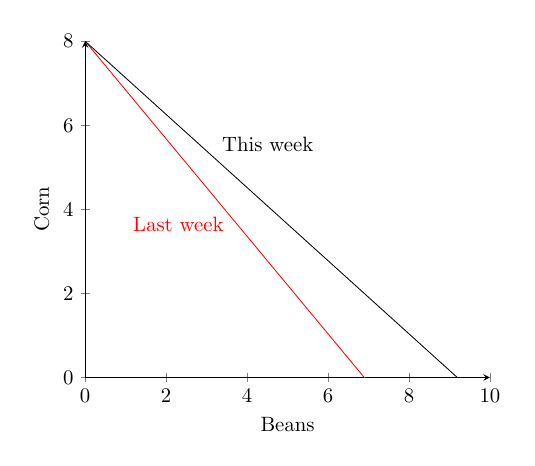
\begin{tikzpicture}[scale=0.75]\begin{axis}[axis lines=left,xmin=0,xmax=10,ymin=0, xlabel=Beans, ylabel=Corn,]
 \addplot[red,domain=0:14.483,samples=4,]{8-1.16*x};
 \draw (axis cs: 3.6,4)node[anchor=north east,red]{Last week};
 \addplot[domain=0:14.5,samples=4,]{8-.87*x};
 \draw(axis cs: 3.2,5.2)node[anchor=south west,]{This week};
 \end{axis}\end{tikzpicture}
		\item \rule{0mm}{0mm}\\ 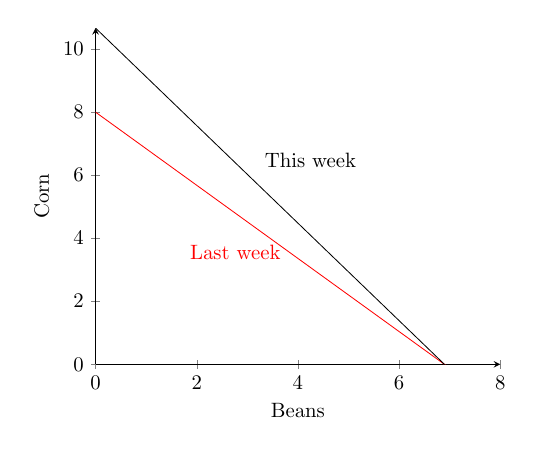
\begin{tikzpicture}[scale=0.75]\begin{axis}[axis lines=left,xmin=0,xmax=8,ymin=0, xlabel=Beans, ylabel=Corn,]
 \addplot[red,domain=0:14.483,samples=4,]{8-1.16*x};
 \draw (axis cs: 3.8,4)node[anchor=north east,red]{Last week};
 \addplot[domain=0:14.5,samples=4,]{10.66667-1.546667*x};
 \draw(axis cs: 3.2,6)node[anchor=south west,]{This week};
 \end{axis}\end{tikzpicture} % 
		\item \rule{0mm}{0mm}\\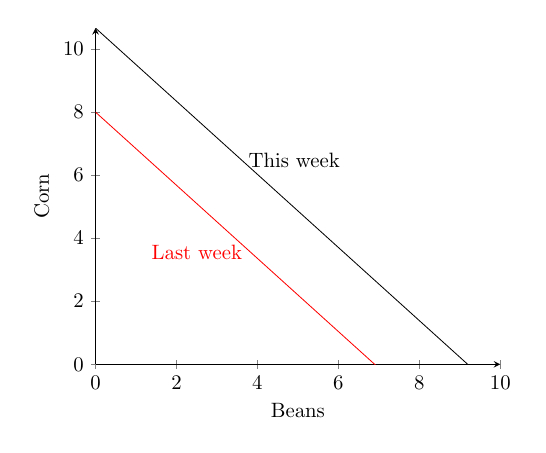
\begin{tikzpicture}[scale=0.75]\begin{axis}[axis lines=left,xmin=0,xmax=10,ymin=0, xlabel=Beans, ylabel=Corn,]
 \addplot[red,domain=0:14.483,samples=4,]{8-1.16*x};
 \draw (axis cs: 3.8,4)node[anchor=north east,red]{Last week};
 \addplot[domain=0:14.5,samples=4,]{10.66667-1.16*x};
 \draw(axis cs: 3.6,6)node[anchor=south west,]{This week};
 \end{axis}\end{tikzpicture} 
		\item \rule{0mm}{0mm}\\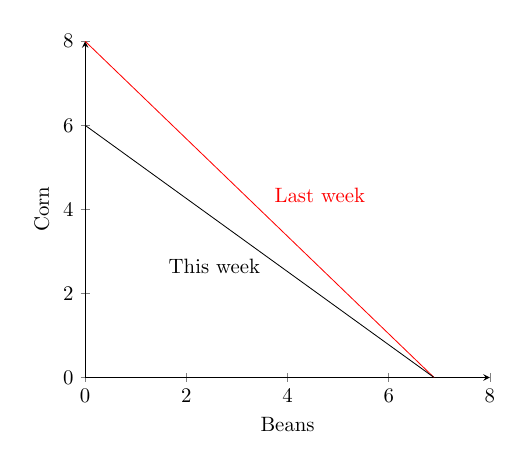
\begin{tikzpicture}[scale=0.75]\begin{axis}[axis lines=left,xmin=0,xmax=8,ymin=0, xlabel=Beans, ylabel=Corn,]
 \addplot[red,domain=0:14.483,samples=4,]{8-1.16*x};
 \draw (axis cs: 3.6,4)node[anchor=south west,red]{Last week};
 \addplot[domain=0:14.5,samples=4,]{6-0.87*x};
 \draw(axis cs: 3.6,3)node[anchor=north east,]{This week};
 \end{axis}\end{tikzpicture}
	\end{enumerate}
\else
\fi

\ifacteven
	\begin{enumerate}[label=\textbf{\Alph*.},itemsep=\fill,align=left]
		\setcounter{enumii}{5}
		\item \rule{0mm}{0mm}\\ 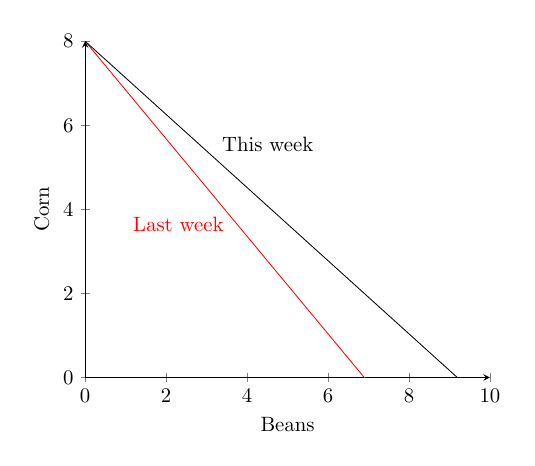
\begin{tikzpicture}[scale=0.75]\begin{axis}[axis lines=left,xmin=0,xmax=10,ymin=0, xlabel=Beans, ylabel=Corn,]
 \addplot[red,domain=0:14.483,samples=4,]{8-1.16*x};
 \draw (axis cs: 3.6,4)node[anchor=north east,red]{Last week};
 \addplot[domain=0:14.5,samples=4,]{8-.87*x};
 \draw(axis cs: 3.2,5.2)node[anchor=south west,]{This week};
 \end{axis}\end{tikzpicture}
		\item \rule{0mm}{0mm}\\ 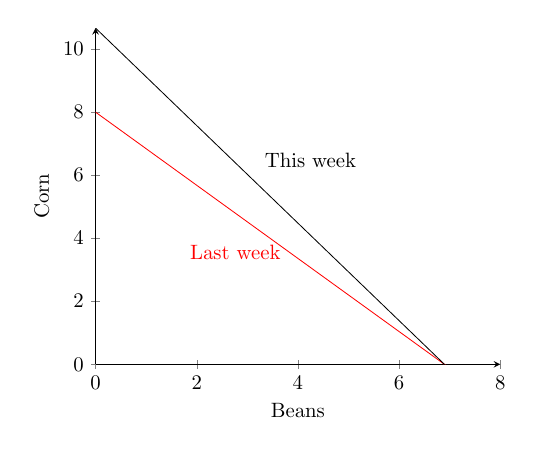
\begin{tikzpicture}[scale=0.75]\begin{axis}[axis lines=left,xmin=0,xmax=8,ymin=0, xlabel=Beans, ylabel=Corn,]
 \addplot[red,domain=0:14.483,samples=4,]{8-1.16*x};
 \draw (axis cs: 3.8,4)node[anchor=north east,red]{Last week};
 \addplot[domain=0:14.5,samples=4,]{10.66667-1.546667*x};
 \draw(axis cs: 3.2,6)node[anchor=south west,]{This week};
 \end{axis}\end{tikzpicture} % 
		\item \rule{0mm}{0mm}\\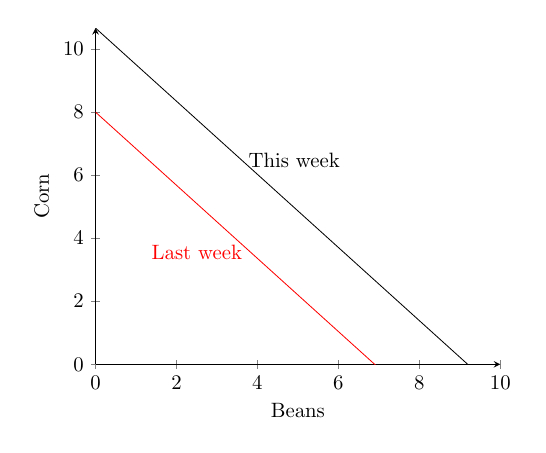
\begin{tikzpicture}[scale=0.75]\begin{axis}[axis lines=left,xmin=0,xmax=10,ymin=0, xlabel=Beans, ylabel=Corn,]
 \addplot[red,domain=0:14.483,samples=4,]{8-1.16*x};
 \draw (axis cs: 3.8,4)node[anchor=north east,red]{Last week};
 \addplot[domain=0:14.5,samples=4,]{10.66667-1.16*x};
 \draw(axis cs: 3.6,6)node[anchor=south west,]{This week};
 \end{axis}\end{tikzpicture} 
		\addtocounter{enumii}{1}
		\item \rule{0mm}{0mm}\\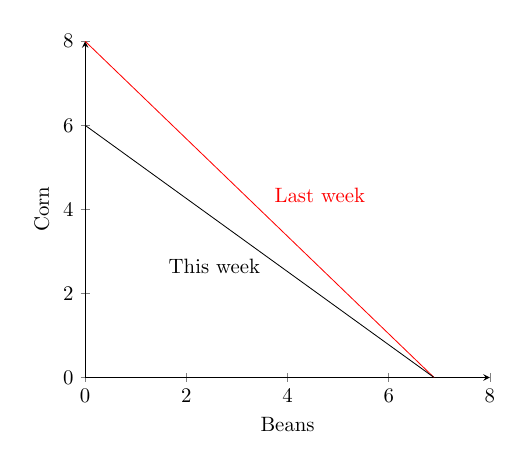
\begin{tikzpicture}[scale=0.75]\begin{axis}[axis lines=left,xmin=0,xmax=8,ymin=0, xlabel=Beans, ylabel=Corn,]
 \addplot[red,domain=0:14.483,samples=4,]{8-1.16*x};
 \draw (axis cs: 3.6,4)node[anchor=south west,red]{Last week};
 \addplot[domain=0:14.5,samples=4,]{6-0.87*x};
 \draw(axis cs: 3.6,3)node[anchor=north east,]{This week};
 \end{axis}\end{tikzpicture}
		\item \rule{0mm}{0mm}\\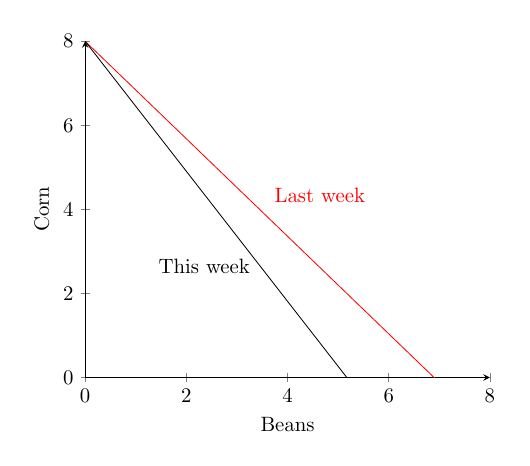
\begin{tikzpicture}[scale=0.75]\begin{axis}[axis lines=left,xmin=0,xmax=8,ymin=0, xlabel=Beans, ylabel=Corn,]
 \addplot[red,domain=0:14.483,samples=4,]{8-1.16*x};
 \draw (axis cs: 3.6,4)node[anchor=south west,red]{Last week};
 \addplot[domain=0:14.5,samples=4,]{8-1.546667*x};
 \draw(axis cs: 3.4,3)node[anchor=north east,]{This week};
 \end{axis}\end{tikzpicture}
	\end{enumerate}
\else
\fi

\ifactodd
	\begin{enumerate}[label=\textbf{\Alph*.},itemsep=\fill,align=left]
		\item \rule{0mm}{0mm}\\ 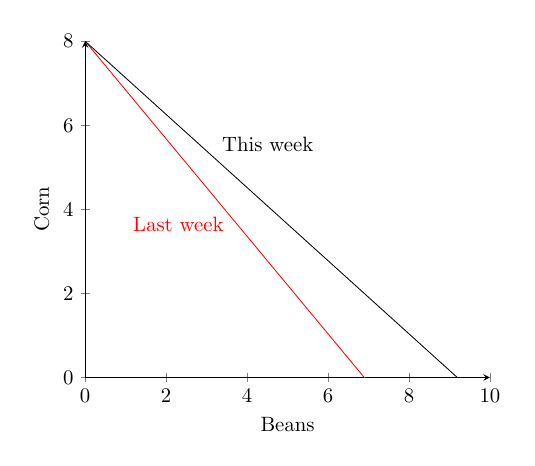
\begin{tikzpicture}[scale=0.75]\begin{axis}[axis lines=left,xmin=0,xmax=10,ymin=0, xlabel=Beans, ylabel=Corn,]
 \addplot[red,domain=0:14.483,samples=4,]{8-1.16*x};
 \draw (axis cs: 3.6,4)node[anchor=north east,red]{Last week};
 \addplot[domain=0:14.5,samples=4,]{8-.87*x};
 \draw(axis cs: 3.2,5.2)node[anchor=south west,]{This week};
 \end{axis}\end{tikzpicture}
		\item \rule{0mm}{0mm}\\ 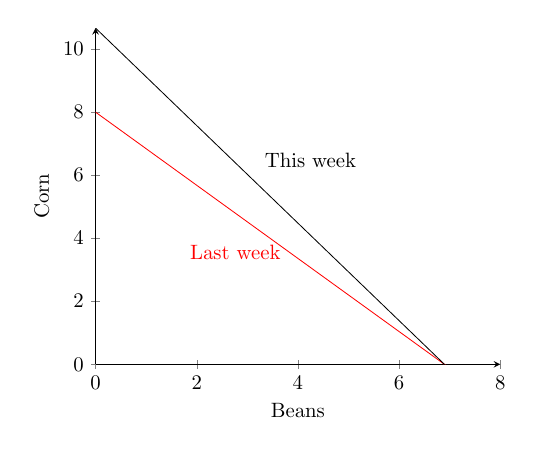
\begin{tikzpicture}[scale=0.75]\begin{axis}[axis lines=left,xmin=0,xmax=8,ymin=0, xlabel=Beans, ylabel=Corn,]
 \addplot[red,domain=0:14.483,samples=4,]{8-1.16*x};
 \draw (axis cs: 3.8,4)node[anchor=north east,red]{Last week};
 \addplot[domain=0:14.5,samples=4,]{10.66667-1.546667*x};
 \draw(axis cs: 3.2,6)node[anchor=south west,]{This week};
 \end{axis}\end{tikzpicture} % 
		\item \rule{0mm}{0mm}\\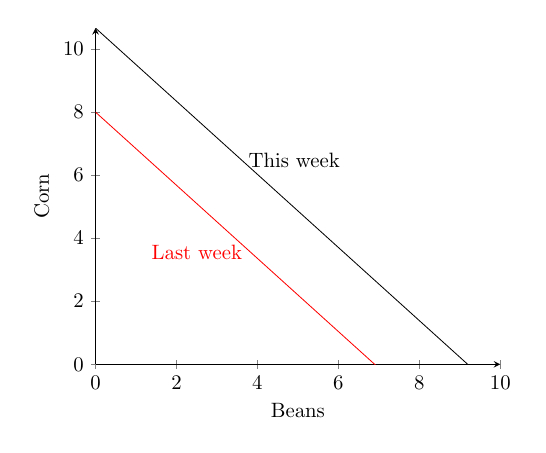
\begin{tikzpicture}[scale=0.75]\begin{axis}[axis lines=left,xmin=0,xmax=10,ymin=0, xlabel=Beans, ylabel=Corn,]
 \addplot[red,domain=0:14.483,samples=4,]{8-1.16*x};
 \draw (axis cs: 3.8,4)node[anchor=north east,red]{Last week};
 \addplot[domain=0:14.5,samples=4,]{10.66667-1.16*x};
 \draw(axis cs: 3.6,6)node[anchor=south west,]{This week};
 \end{axis}\end{tikzpicture} 
		\item \rule{0mm}{0mm}\\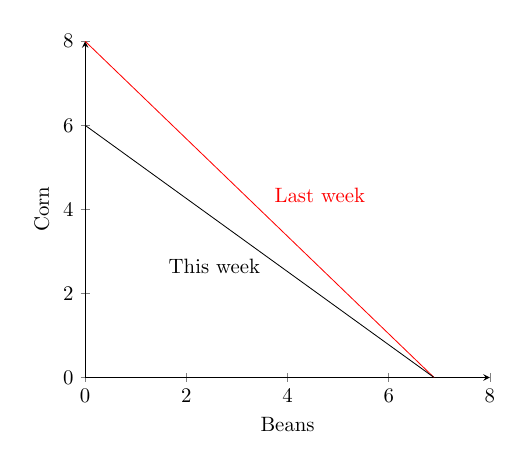
\begin{tikzpicture}[scale=0.75]\begin{axis}[axis lines=left,xmin=0,xmax=8,ymin=0, xlabel=Beans, ylabel=Corn,]
 \addplot[red,domain=0:14.483,samples=4,]{8-1.16*x};
 \draw (axis cs: 3.6,4)node[anchor=south west,red]{Last week};
 \addplot[domain=0:14.5,samples=4,]{6-0.87*x};
 \draw(axis cs: 3.6,3)node[anchor=north east,]{This week};
 \end{axis}\end{tikzpicture}
		\item \rule{0mm}{0mm}\\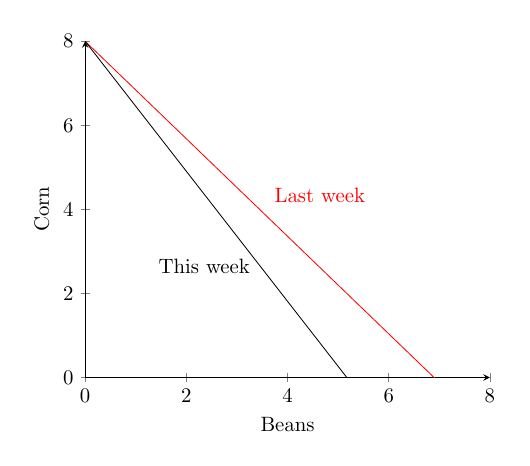
\begin{tikzpicture}[scale=0.75]\begin{axis}[axis lines=left,xmin=0,xmax=8,ymin=0, xlabel=Beans, ylabel=Corn,]
 \addplot[red,domain=0:14.483,samples=4,]{8-1.16*x};
 \draw (axis cs: 3.6,4)node[anchor=south west,red]{Last week};
 \addplot[domain=0:14.5,samples=4,]{8-1.546667*x};
 \draw(axis cs: 3.4,3)node[anchor=north east,]{This week};
 \end{axis}\end{tikzpicture}
	\end{enumerate}
\else
\fi

\ifgridin
 \rule{0mm}{0mm}\\ 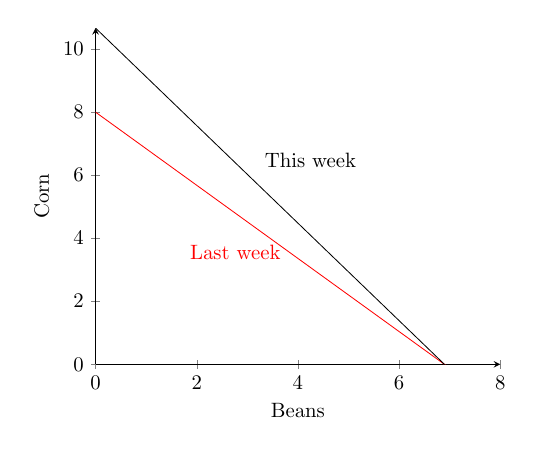
\begin{tikzpicture}[scale=0.75]\begin{axis}[axis lines=left,xmin=0,xmax=8,ymin=0, xlabel=Beans, ylabel=Corn,]
 \addplot[red,domain=0:14.483,samples=4,]{8-1.16*x};
 \draw (axis cs: 3.8,4)node[anchor=north east,red]{Last week};
 \addplot[domain=0:14.5,samples=4,]{10.66667-1.546667*x};
 \draw(axis cs: 3.2,6)node[anchor=south west,]{This week};
 \end{axis}\end{tikzpicture} % 
		
\else
\fi

